%Version 2.1 April 2023
% See section 11 of the User Manual for version history
%
%%%%%%%%%%%%%%%%%%%%%%%%%%%%%%%%%%%%%%%%%%%%%%%%%%%%%%%%%%%%%%%%%%%%%%
%%                                                                 %%
%% Please do not use \input{...} to include other tex files.       %%
%% Submit your LaTeX manuscript as one .tex document.              %%
%%                                                                 %%
%% All additional figures and files should be attached             %%
%% separately and not embedded in the \TeX\ document itself.       %%
%%                                                                 %%
%%%%%%%%%%%%%%%%%%%%%%%%%%%%%%%%%%%%%%%%%%%%%%%%%%%%%%%%%%%%%%%%%%%%%

%%\documentclass[referee,sn-basic]{sn-jnl}% referee option is meant for double line spacing

%%=======================================================%%
%% to print line numbers in the margin use lineno option %%
%%=======================================================%%

%%\documentclass[lineno,sn-basic]{sn-jnl}% Basic Springer Nature Reference Style/Chemistry Reference Style

%%======================================================%%
%% to compile with pdflatex/xelatex use pdflatex option %%
%%======================================================%%

%%\documentclass[pdflatex,sn-basic]{sn-jnl}% Basic Springer Nature Reference Style/Chemistry Reference Style


%%Note: the following reference styles support Namedate and Numbered referencing. By default the style follows the most common style. To switch between the options you can add or remove ?Numbered? in the optional parenthesis.
%%The option is available for: sn-basic.bst, sn-vancouver.bst, sn-chicago.bst, sn-mathphys.bst. %

\documentclass[pdflatex,referee,lineno,sn-nature]{sn-jnl}% Style for submissions to Nature Portfolio journals
%%\documentclass[sn-basic]{sn-jnl}% Basic Springer Nature Reference Style/Chemistry Reference Style
%%\documentclass[sn-mathphys,Numbered]{sn-jnl}% Math and Physical Sciences Reference Style
%%\documentclass[sn-aps]{sn-jnl}% American Physical Society (APS) Reference Style
%%\documentclass[sn-vancouver,Numbered]{sn-jnl}% Vancouver Reference Style
%%\documentclass[sn-apa]{sn-jnl}% APA Reference Style
%%\documentclass[sn-chicago]{sn-jnl}% Chicago-based Humanities Reference Style
%%\documentclass[default]{sn-jnl}% Default
%%\documentclass[default,iicol]{sn-jnl}% Default with double column layout

%%%% Standard Packages
%%<additional latex packages if required can be included here>

\usepackage{graphicx}%
\usepackage{multirow}%
\usepackage{amsmath,amssymb,amsfonts}%
\usepackage{amsthm}%
\usepackage{mathrsfs}%
\usepackage[title]{appendix}%
\usepackage{xcolor}%
\usepackage{textcomp}%
\usepackage{manyfoot}%
\usepackage{booktabs}%
\usepackage{algorithm}%
\usepackage{algorithmicx}%
\usepackage{algpseudocode}%
\usepackage{listings}%
%%%%

%% Added by LA/RC
%%   NOTE: to compile, use tinytex::pdflatex("kalis.tex", clean = FALSE)
%%         in order to preserve .aux for cross-referencing
\let\proglang=\textsf
\newcommand{\pkg}[1]{{\fontseries{m}\fontseries{b}\selectfont #1}}
\usepackage{cleveref}
\usepackage{anyfontsize}
%% /Added by LA/RC

\raggedbottom
%%\unnumbered% uncomment this for unnumbered level heads


\begin{document}

\title[kalis: Local Ancestry Inference in R]{kalis: A Modern Implementation of the Li \& Stephens Model for Local Ancestry Inference in R}

%% Affiliations

\author*[1]{\fnm{Louis J.M.} \sur{Aslett}}\email{louis.aslett@durham.ac.uk}

\author[2]{\fnm{Ryan R.} \sur{Christ}}\email{ryan.christ@yale.edu}

\affil*[1]{\orgdiv{Department of Mathematical Sciences}, \orgname{Durham University}, \orgaddress{\street{Stockton Road}, \city{Durham}, \postcode{DH1 3LE}, \state{County Durham}, \country{UK}}}

\affil[2]{\orgdiv{Department of Genetics}, \orgname{Yale School of Medicine}, \orgaddress{\street{333 Cedar Street}, \city{New Haven}, \postcode{06520}, \state{CT}, \country{USA}}}


%% Abstract

\abstract{\textbf{Background}
Approximating the recent phylogeny of $N$ phased haplotypes at a set of variants along the genome is a core problem in modern population genomics and central to performing genome-wide screens for association, selection, introgression, and other signals.
The Li \& Stephens (LS) model provides a simple yet powerful hidden Markov model for inferring the recent ancestry at a given variant, represented as an $N \times N$ distance matrix based on posterior decodings.
However, existing posterior decoding implementations for the LS model cannot scale to modern datasets with tens or hundreds of thousands of genomes.

\textbf{Results}
We provide a high-performance engine to compute the LS model, enabling users to rapidly develop a range of variant-specific ancestral inference pipelines on top, exposed via an easy to use package, \pkg{kalis}, in the statistical programming language \proglang{R}.
\pkg{kalis} exploits both multi-core parallelism and modern CPU vector instruction sets to enable scaling to problem sizes that would previously have been prohibitively slow to work with.

\textbf{Conclusions}
The resulting distance matrices accessible via \pkg{kalis} enable local ancestry, selection, and association studies in modern large scale genomic datasets.}

\keywords{Li \& Stephens Model, R package, probabilistic haplotype model, Hidden Markov Model, genomics, high performance computation}

%%\pacs[JEL Classification]{D8, H51}

%%\pacs[MSC Classification]{35A01, 65L10, 65L12, 65L20, 65L70}

\maketitle

\section*{Background}
\label{introduction}

The hidden Markov model (HMM) of haplotype diversity proposed by Li \& Stephens \cite{Li2213} (hereinafter, the LS model) has become the basis for several probabilistic phasing, ancestry inference, and demographic inference methods in modern genomics \cite{speidel,Song1005}.
The LS model provides the basis for the genome-wide ancestry inference software ChromoPainter, which summarizes the ancestry of \(N\) haplotypes with an \(N \times N\) similarity matrix \cite{lawson2012inference}.
This matrix is obtained by running \(N\) independent HMMs in which each haplotype is modelled as a mosaic of all of the other haplotypes in the sample.
This \emph{`all-vs-all'} copying approach is motivated by the product of approximate conditionals (PAC) likelihood originally proposed by \cite{Li2213} and allows ChromoPainter to render a chromosome-wide estimate of the recent ancestry of the \(N\) haplotypes with high resolution.

Beyond chromosome-wide summaries, the LS model can also be used for variant-specific ancestry inference.
The contemporary importance of this is highlighted by the recent advances achieved in the RELATE software suite \cite{speidel}, which uses the LS model internally to initialise variant-specific ancestral trees for downstream population genetic analyses ranging from demography to selection inference.
\pkg{kalis} focuses on providing a high-performance engine to compute exclusively the LS model, enabling users to rapidly develop a range of future variant-specific ancestral inference pipelines on top, in the easy to use statistical programming language \proglang{R} \cite{R}.

At the same time, it has been recognised for over a decade \cite{sutter2005free} that the serial execution speed of CPUs will increase modestly, with additional performance primarily coming from concurrency via multi-core architectures or the growing width of specialised single instruction, multiple data (SIMD) instruction sets.
Whilst multi-core architectures are now somewhat routinely exploited via forked processes or threading, SIMD instructions remain an often overlooked source of performance gains, possibly because they are harder to program.
There are a cornucopia of SIMD instruction sets: on the Intel platform the genesis was in the 64-bit wide MMX instruction set \cite{mmx} which allows simultaneous operation on two 32-bit, four 16-bit or eight 8-bit integers.
The most recent incarnation on Intel CPUs is a suite of AVX-512 instruction sets \cite{intelisa}, now capable of operating on 512-bits of various data types simultaneously (eg eight 64-bit floating point, or sixteen 32-bit integer values).
Other CPU designs have similar SIMD technologies, such as NEON on ARM CPU \cite{armneon} designs (including the Apple M1 and M2 processors, as well as Amazon Web Services Graviton range).
Additionally all modern CPUs are superscalar architectures supporting instruction level parallelism, an advance that has been in the consumer Intel platform since the Pentium \cite{pentium}.
Judicious programming can make it easier for compilers and the deep reorder buffers of modern pipelined CPUs to exploit this more hidden form of parallelism.

In this work we provide a reformulation of the LS model and an optimised memory representation for haplotypes, which together enable us to leverage \emph{both} multi-core and SIMD vector instruction parallelism to obtain local genetic distance matrices for problem sizes that previously appeared out of reach.
This high performance implementation is programmed in \proglang{C} \cite{C18}, with an easy to use interface provided in \proglang{R} \cite{R}.
We provide low-level targets of AVX2, AVX-512 and NEON instruction sets (covering the vast majority of CPUs in use today), and the whole package has an extensive suite of \(162,835\) unit tests.

In the Implementation section below, we start with a description of the LS model and our reformulation which makes it amenable to these high-performance CPU technologies.
We also describe the technical details of the underlying low-level implementation for the interested reader.
We then demonstrate the performance that can be achieved with \pkg{kalis}, including examples with 100,000 haplotypes capable of running on a single machine.
To the best of our knowledge, this is the first example of running the LS model at the scale of hundreds-of-thousands of haplotypes.
We also present a real data example using \pkg{kalis} to examine the ancestry at the \emph{LCT} gene.
In the following Discussion section, we describe the user friendly \proglang{R} interface which enables easy use of the high performance implementation without any knowledge of the underlying CPU technologies.



\section*{Implementation}

\subsection*{The LS model}
\label{sec:lsmodel}

To formalize our objective, let \(h\) be an \(L \times N\) matrix of \(0\)s and \(1\)s encoding \(N\) phased haplotypes at \(L\) sites.
Let \(h_i^{\ell} \in \{0,1\}\) denote the the \((\ell,i)\)th element of \(h\).
For brevity, let \(h_i\) denote the \(i\)th haplotype (the \(i\)th column of \(h\)) and \(h_{-i}\) denote all of the haplotypes excluding the \(i\)th haplotype.
The LS model proposes an HMM for \(h_i | h_{-i}\) in which the hidden state at variant \(\ell\), \(X^{\ell}_i \in \{1,\dots,N\} \setminus i\), is an index indicating the haplotype in \(h_{-i}\) that \(h_i\) is most closely related to (or ``copies from'') at variant \(l\).
We present here their proposed emission and transition kernels (see Equation A1 and Equation A2 in \cite{Li2213}) with a simplified parametrisation that is similar, but not identical, to that used by ChromoPainter.

While the original LS model assumes that each haplotype has an equal \emph{a priori} probability of copying from any other, following ChromoPainter, we define a left stochastic matrix of prior copying probabilities \(\Pi \in \mathbb{R}^{N \times N}\) where \(\Pi_{ji}\) is the prior probability that haplotype \(j\) is copied by \(i\) and, by convention, \(\Pi_{ii} = 0\).
Here and whenever possible in \pkg{kalis}, all matrices are column-oriented such that the \(i\)th column pertains to an independent HMM where \(h_i\) is treated as the observation.
There is some probability of a mis-copy at variant \(\ell\), \(\mu^{\ell}\), which under the LS model is set proportional to the mutation rate at \(\ell\).
This leads to an emission kernel of the form
\begin{equation}
	\theta_{ji}^{\ell} := \mathbb{P}\left(h_{i}^\ell \left| X_{i}^{\ell} = j \right. \right)
	= \begin{cases}
		1 - \mu^{\ell} & \text{if } h_{i}^\ell = h_j^\ell \\
		\mu^{\ell} & \text{if } h_{i}^\ell \neq h_j^\ell \\
	\end{cases} .
	\label{eq:emission}
\end{equation}

The transition kernel between hidden states is based on the recombination rate between sites.
Let \(m^l\) be the genetic distance between variant \(l\) and variant \(l+1\) in Morgans (the expected number of recombination events per meiosis).
Define \(N_e = 4\tilde{N_e}/N\) where \(\tilde{N_e}\) is the effective diploid population size (ie half of the haploid effective population size).
Then, under the LS model the transition kernel is
\begin{equation}
	P(X_{i}^\ell = k | X_{i}^{\ell-1} = j)
	= \Pi_{ki} \rho^\ell + \mathbf{1}\left\{k = j\right\} \left(1-\rho^\ell\right) ,
	\label{eq:transition}
\end{equation}
where \(\rho^\ell = 1-\exp\left(-N_e m^\ell\right)\) and \(\mathbf{1}\left\{\cdot\right\}\) is the indicator function.
\cite{Li2213} observe that in practice the estimation of recombination rates is improved when the scaled recombination rate is raised to a power, so we adopt this approach and introduce an exponent \(\gamma\).
For \(\gamma>1\) the recombination map becomes more heavily peaked, whereas \(\gamma<1\) tempers the recombination map to make it more flat and smooth.
Hence, in \pkg{kalis}, we set
\begin{equation}
	\rho^\ell := 1-\exp\left(-N_e \left(m^\ell\right)^\gamma\right), \label{eq:rho}
\end{equation}
calculated using \texttt{expm1()} to help avoid underflow.

In keeping with the nomenclature introduced by \cite{lawson2012inference}, we refer to \(h_i\) as the ``recipient haplotype'' and the remaining haplotypes, \(h_{-i}\), as the ``donor haplotypes'', in the context of the HMM where \(h_{i}\) is treated as the emitted observation vector.
This reflects the fact that each recipient haplotype \(h_i\) is modelled as an imperfectly copied mosaic of the other observed haplotypes under the LS model.
Hence, the posterior marginal probability at variant \(\ell\), \(p^{\ell}_{ji} := \mathbb{P}\left(\left. X_i^\ell = j \right| h\right)\), is the probability that donor \(j\) is copied by recipient \(i\) at variant \(\ell\) given the haplotypes \(h\).
Under the above definitions of the prior copying probabilities \(\Pi\), the emission kernel \eqref{eq:emission}, and the transition kernel \eqref{eq:transition}, the full \(N \times N\) matrix of copying probabilities at \(\ell\), \(p^\ell\), can be obtained by running the standard forward and backward recursions \cite{rabiner1989tutorial} for each column (ie for each independent HMM).

From these posterior probabilities, we calculate a local \(N \times N\) distance matrix, \(d^\ell\).
Firstly, notice that theoretically \(p_{ij}^\ell > 0\), but it can be that \(p_{ij}^\ell < \varepsilon\), where \(\varepsilon\) is the double precision machine epsilon (\(\approx 2.22\times10^{-16}\), \cite{C18}, pp.26).
Effectively this means \(d_{ij}^\ell\) is too large to reliably work with precisely, and so for the purposes of distance calculations we treat \(\varepsilon\) as the smallest observable posterior probability, yielding \begin{equation}
	d_{ji}^\ell = -\frac{\log\left(p_{ji}^\ell \vee \varepsilon \right) + \log\left(p_{ij}^\ell \vee \varepsilon  \right)}{2} \quad \forall\ j \neq i \label{eq:distmat}
\end{equation}
where \(\vee\) is the maximum binary operator.
By convention \(d_{ii} = 0\) for all \(i\).

We proceed in the next Section to reformulate the forward and backward recursions so that we can more fully exploit modern high-performance CPU instruction sets, while preserving numerical precision.



\subsection*{Modification of the forward-backward algorithm}
\label{sec:reformulation}

The \(N\) independent HMMs of the LS model have forward and backward probabilities, respectively: \begin{equation*}
	\tilde{\alpha}_{ji}^{\ell} = \mathbb{P}\left( X_i^\ell = j, h_i^{1:\ell} \right), \qquad
	\tilde{\beta}_{ji}^{\ell} = \mathbb{P}\left(\left.  h_i^{\ell+1 : L}  \right| X_i^\ell = j \right), \qquad i \in \{1,\dots,N\} ,
\end{equation*}
where \(h_{i}^{1:\ell}\) denotes haplotype \(i\) from variant \(1\) to \(\ell\) inclusive.

Define,
\begin{align}
	F_i^\ell &:= \sum_{j=1}^N \tilde{\alpha}_{ji}^{\ell} & F_i^{0} &:= 1 \label{eq:F} \\
	G_i^\ell &:= \sum_{j=1}^N \tilde{\beta}_{ji}^{\ell+1}\theta_{ji}^{\ell+1} \pi_{ji} & G_i^L &:= 1 \label{eq:G}
\end{align}
Then the forward and backward recursions for the LS model can be written in vector notation (subscript \(\cdot\) denoting a vectorised index),
\begin{align}
	\tilde{\alpha}_{\cdot i}^{\ell} &\gets \theta^{\ell}_{\cdot i} \left( \left(1-\rho^{\ell-1}\right) \tilde{\alpha}_{\cdot i}^{\ell-1} + \rho^{\ell-1} F_i^{\ell-1} \pi_{\cdot i} \right) & \text{for } \ell &\in \{2,\dots,L\}, \label{eq:raw_forward} \\
	\tilde{\beta}_{\cdot i}^{\ell} &\gets \left( 1- \rho^{\ell}\right) \tilde{\beta}_{\cdot i}^{\ell+1} \theta^{\ell+1}_{\cdot i} + \rho^{\ell} G_i^\ell & \text{for } \ell &\in \{1,\dots,L-1\} \label{eq:raw_backward}.
\end{align}
with recursions initialised with \(\alpha_{\cdot i}^{1} \gets \theta^{1}_{\cdot i} \pi_{\cdot i}\) and \(\beta_{\cdot i}^{L} \gets 1\).
Note that \Cref{eq:raw_forward} corresponds to Equation A5 in \cite{Li2213}.

To partially mitigate the risk of underflow, the forward recursion can be rearranged in terms of \(\alpha_{\cdot i}^{\ell} := \frac{\tilde{\alpha}_{\cdot i}^{\ell}}{ F_i^{\ell-1}}\), and the backward recursion in terms of \(\beta_{\cdot i}^{\ell} := \frac{\tilde{\beta}_{\cdot i}^{\ell}}{G_i^{\ell}}\) (see the Appendix (Additional file 1) for details).
Thus, in full for \(\ell \in \{1,\dots,L\}\) we compute,
\begin{align}
	\alpha_{\cdot i}^{1} &\gets \theta^{1}_{\cdot i} \pi_{\cdot i} &\textrm{for} \quad \ell = 1 \label{eq:fwd0} \\
	\alpha_{\cdot i}^{\ell} &\gets \theta^{\ell}_{\cdot i} \left( \left(1-\rho^{\ell-1}\right) \frac{\alpha_{\cdot i}^{\ell-1}}{\underset{j}{\sum} \alpha_{ji}^{\ell-1}} + \rho^{\ell-1} \pi_{\cdot i} \right) &\textrm{for} \quad \ell > 1 \label{eq:fwd1} \\ \intertext{and}
	\beta_{\cdot i}^{L} &\gets 1 &\textrm{for} \quad \ell = L \label{eq:bck0} \\
	\beta_{\cdot i}^{\ell} &\gets \left( 1- \rho^{\ell}\right) \frac{\beta_{\cdot i}^{\ell+1} \theta^{\ell+1}_{\cdot i}}{\underset{j}{\sum} \beta_{ji}^{\ell+1}\theta_{ji}^{\ell+1} \pi_{ji}} + \rho^\ell &\textrm{for} \quad \ell < L \label{eq:bck1}
\end{align}

Given \(\alpha_{\cdot i}^\ell\) and \(\beta_{\cdot i}^\ell\), the vector of posterior probabilities for recipient \(i\), \(p^\ell_{\cdot i}\), can be calculated directly by normalising,
\begin{equation}
	p^\ell_{\cdot i} = \frac{\alpha^\ell_{\cdot i} \odot \beta^\ell_{\cdot i}}{\sum\limits_j \alpha^\ell_{ji} \odot \beta^\ell_{ji}} \label{eq:postprob}
\end{equation}
where \(\odot\) denotes the Hadamard product.
In the event that \(\sum\limits_j \alpha^\ell_{ji} \odot \beta^\ell_{ji} = 0\), the distance between the recipient haplotype \(i\) and all of the donor haplotypes is beyond numerical precision, so as per the earlier discussion we define \(p_{ji}^\ell = \varepsilon \ \forall\ j \ne i\).

Finally, the local distances follow by taking the negative log and symmetrising.
Note that if the distances are standardised for one of these columns, to account for the fact that the standard deviation will be 0, we set all of the standardised distances to 0.
Please see the Appendix (Additional file 1) for a discussion on parameter values and exactly how \pkg{kalis} performs certain computations to maintain the numerical stability of the algorithm.



\subsection*{Core Implementation Details}
\label{sec:core}

The \proglang{R} interface described hereinbefore is a thin wrapper layer around a high-performance implementation of the core algorithm which is written in standards compliant C18 \cite{C18}.
Most data structures are represented with native \proglang{R} types enabling user inspection and manipulation, except for the haplotype sequences themselves.

Computationally, the innermost forward and backward recursions are implemented using compiler intrinsics to exploit a variety of modern CPU instruction sets, including Streaming SIMD Extensions (SSE2 and SSE4.1), Advanced Vector Extensions (AVX, AVX2, AVX-512 and FMA) and Bit Manipulation Instructions (BMI2) on Intel platforms; as well as NEON on ARM platforms.
AVX2 is supported in Intel CPUs of the Haswell generation (released Q2 of 2013) or later, AVX-512 tends to be available only in recent Intel server and workstation grade CPUs, and NEON is available for ARM Cortex-A and Cortex-R series CPUs, as well as Apple M1/M2 and Amazon Web Services Graviton processors.
Although this covers most CPUs likely to be in use today, we none-the-less provide reference implementations in pure standards compliant \proglang{C} which will operate on any CPU architecture with a C18 compliant compiler.
During package compilation, the correct code-paths are compiled based on detection of the presence or absence of the required instruction sets, or at the direction of the user via compiler flags.
See the Appendix (Additional file 1) for more details, and for guidance on how to directly check your CPU for SIMD support.

It may be worth noting at this juncture that it was an explicit design choice to target CPUs and not GPU or tensor cards initially.
This is because most University high performance computing clusters have plentiful CPU resources, often with untapped power in advanced SIMD instructions sets.
We believe that the problem size that can be realistically tackled in many genetics studies can be massively increased \emph{without} needing to resort to add-on cards, though to scale beyond even this we may explore heterogeneous computing architectures in future \pkg{kalis} research.

In this section, we now describe the inner workings and design principles of the package, first covering in detail the data structures (both user facing and internal), followed by the computational implementation.



\subsection*{Data structures}
\label{data-structures}

There are three user accessible data structures utilised in the package and a low level binary haplotype representation which is not directly user accessible.
The two principle data structures of interest to users are forward and backward table objects, represented as native \proglang{R} lists with respective S3 class names \texttt{kalisForwardTable} and \texttt{kalisBackwardTable} (detailed in Table \ref{tab:fwdbck} and discussed later), which are created with package functions \texttt{MakeForwardTable()} and \texttt{MakeBackwardTable()} respectively.
The third user accessible data structure holds the LS model parameters, represented as a native \proglang{R} environment with S3 class name \texttt{kalisParameters}, which can be created with the package function \texttt{Parameters()}.



\subsubsection*{Haplotype data}
\label{sec:haplotypedata}

The haplotypes are stored in an optimised binary representation which is only natively accessible from within C.
Note that here ``optimised'' is not a reference to space-optimisation: it would be possible to represent the haplotypes in an even more compressed manner, but we aim for streaming compute speed optimisation instead.

The haplotypes are loaded from disk and transformed to an in memory cache in this representation via \texttt{CacheHaplotypes()}, but this function does not return any handle to the loaded data.
Thus the package provides the accessor function \texttt{QueryCache()}, which copies genome segments from the binary representation into native \proglang{R} integer vectors for user inspection.

When \texttt{CacheHaplotypes()} loads haplotypes into the cache, they are interleaved into a flat memory space which is organised as variant-major.
That is, variant 1 of each haplotype is loaded, converted to a binary 0/1 and then 32 consecutive haplotypes are packed into an unsigned integer.
Moreover, the initial flat memory allocation is aligned on a 32-byte boundary to satisfy memory alignment requirements for some CPU vector instructions\footnote{Certain modern CPUs do not require specific alignment to be able to load memory to SSE/AVX registers, but for maximum compatibility we honor the alignment anyway.}, and after all haplotypes at a given variant are packed into consecutive unsigned integers the pointer is wound forward to the next 32-byte boundary to ensure the next variant starts on an SSE/AVX vector compatible memory boundary.
This is depicted in Figure \ref{fig:hapsmem}.

\begin{figure}
  \centering
  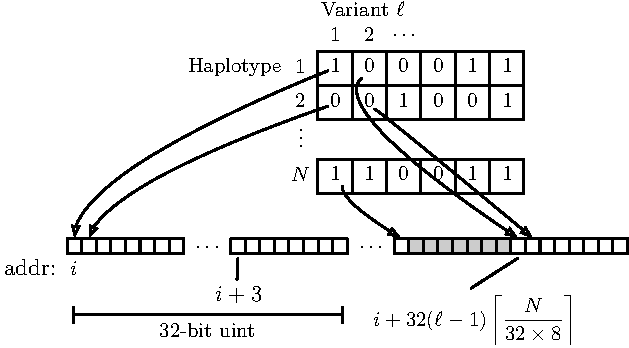
\includegraphics{fig1}
  \caption{
    Efficient binary representation of interleaved haplotypes in memory, with 32-byte boundary alignment for each variant start for SSE/AVX instructions (here $i \mod 32 = 0$).
    The grey boxes indicate essentially `wasted' bits which are ignored to ensure alignment for the start of the next variant.
  }
  \label{fig:hapsmem}
\end{figure}

Firstly, note that this orientation is natural, since the forward and backward recursions operate variant by variant, meaning variant-major storage ensures sequential memory locations are fetched during a recursion.
Indeed, with the cache line size of 64-bytes (starting Intel Pentium IV), we essentially trigger the loading of \(64 \times 8 = 512\) neighbouring variants upon accessing the first variant in a recursion.
This effect is even more pronounced on Apple M1/M2 whose cache line size is 128-bytes, resulting in 1024 variants being pre-fetched upon access to the first variant in a recursion.

Secondly, a possible drawback is that we must extract the individual bit into a double floating point representation in order to compute with it in the recursion.
However, efficient CPU instructions can help here too: take for example the following strategy \pkg{kalis} uses on an AVX2 capable CPU.
Using the \texttt{PDEP} instruction in BMI2, we can efficiently deposit a bit into every ninth bit of an \texttt{int} (so there are now 4 8-bit integers taking on the value of the haplotype at this variant packed in an \texttt{int}).
Then, using SSE2, SSE4.1 and AVX instructions one can inflate through representations from 4 8-bit integers packed in an \texttt{int} up to 4 64-bit doubles packed in a 256-bit AVX register.
As such, we are then ready to operate with this variant in parallel using AVX instructions.

During development, testing indicated the memory bandwidth and cache efficiency savings of the packed binary representation provided speed-ups thanks to these instructions efficiently enabling unpacking and spreading a haplotype variant bit for parallel use.
Furthermore, such a compact representation means that more of L1/L2 cache and memory bus bandwidth is left available for forward and backward tables, which are the largest objects we work with in this problem.



\subsubsection*{Parameters}
\label{parameters}

The \texttt{kalisParameters} object uses an environment rather than list for parameters for two reasons: (i) the parameter environment and its bindings are locked which prevents changes in parameter values between forward or backward table propagation steps, since parameters must be fixed for all steps of a given forward or backward computation; and (ii) an environment explicitly ensures the (often large) parameter vectors are not copied when associated with potentially many different tables, but will always be purely referenced.

The environment contains only two members: another environment with the actual parameter values (which is locked with \texttt{lockEnvironment()}); and a SHA-256 hash of those parameter values (details in Table \ref{tab:pars}).
The purpose of the hash is to be able to efficiently determine whether the correct parameter set for a given forward or backward table has been passed when computing forward or backward recursions from an already initialised table (since it would be incorrect to propagate forward or backward using different parameter sets in different parts of the genome).

\begin{table}[tbp]
	\centering
	\begin{tabular}{l|ll}
		\hline
		\texttt{kalisParameters} object & Data type & \\ \hline\hline
		\texttt{pars} & Locked \proglang{R} environment, containing: \\
		& \texttt{rho} & vector length $L$ \\
		& \texttt{mu} & vector length $L$, or scalar \\
		& \texttt{Pi} & $N \times N$ matrix, or scalar \\
		\texttt{sha256} & character & \\ \hline
	\end{tabular}
	\caption{The content of the data structure representing parameter objects.}
	\label{tab:pars}
\end{table}



\subsubsection*{Forward/backward tables}
\label{forwardbackward-tables}

\begin{table}[tbp]
	\centering
	\begin{tabular}{ll|ll|l}
		\hline
		\multicolumn{2}{l|}{\texttt{kalisForwardTable} object} &   \multicolumn{2}{l|}{\texttt{kalisBackwardTable} object} & Data type \\ \hline\hline
		\texttt{alpha} & $= \alpha^\ell_{\cdot\cdot}$ & \texttt{beta} & $= \beta^\ell_{\cdot\cdot}$  & $N   \times N$ matrix \\
		\texttt{alpha.f} & $= F^\ell$ & \texttt{beta.g} & $= G^\ell$ & vector length $N$ \\
		\texttt{l} & $= \ell$ & \texttt{l} & $= \ell$ & integer scalar \\
		\texttt{from\_recipient} & & \texttt{from\_recipient} & & integer scalar \\
		\texttt{to\_recipient} & & \texttt{to\_recipient} & & integer scalar \\
		\texttt{pars.sha256} & & \texttt{pars.sha256} & & character \\
		& & \texttt{beta.theta} & & logical scalar \\ \hline
	\end{tabular}
	\caption{The content of the core data structures representing forward and backward table objects, together with their correspondence to mathematical quantities.}
	\label{tab:fwdbck}
\end{table}

Recall that the recipients (columns) in the forward/backward tables correspond to independent HMMs.
Therefore, \pkg{kalis} enables storing only a `slice' of recipients in a forward/backward table, making parallelisation across non-shared memory clusters much simpler: given all haplotype data, these recipient slices can be independently propagated in a communication free manner.

The forward and backward table objects contain not only the (upto) \(N\) independent forward/backward vectors at variant \(\ell\), but also supporting meta-data.
This includes the variant the table is currently at, the scaling constants \(F^\ell\) (forward, \Cref{eq:F}) or \(G^\ell\) (backward, \Cref{eq:G}), the range of recipient haplotypes represented (that is, the recipient HMMs to which the column corresponds), and a hash of the parameter values used in propagating this table.

In total, a full-size forward table for example requires \(8N^2+8N+1576\) bytes of memory\footnote{Measured under \proglang{R} 4.2.2} for storage and the small overhead of \proglang{R} object management.
Since this grows quadratically in the number of haplotypes, most functions in the package operate on forward and backward table objects in-place, rather than via the idiomatic copy-on-write mechanism of standard \proglang{R}.
The most important consequence of this for users is that standard assignment of a table object to another variable name only creates a reference and so an explicit copy must be made by using the \texttt{CopyTable()} utility function provided in the package.



\subsection*{Core SIMD code}
\label{core-simd-code}

The two most important core algorithms which are accelerated with SIMD vector instructions are the forward and backward recursions.
This code is fully implemented in \proglang{C}, with tailored modifications accounting for all combinations of: scalar/vector \(\mu\), scalar/matrix \(\Pi\), and use of the asymmetric mutation model of RELATE \cite{speidel} or not (ie 8 combinations); to ensure that minimal memory accesses are performed where possible.
So, for example, scalar \(\mu\) and scalar \(\Pi\) parameters will be faster than any other combination since these values are likely to be held in registers (or at least L1 cache) for the duration of the recursion.

Additionally, in all places where we identify SIMD instructions may be used, a macro is deployed, with a header file providing all mappings from these macros to a specific SIMD instruction for all supported instruction sets.
Taking arguably the simplest non-trivial example, all \texttt{src/ExactForward*.c} and \texttt{src/ExactBackward*.c} files make us of the custom macro \texttt{KALIS\_MUL\_DOUBLE(X,\ Y)} when they need to multiply \texttt{KALIS\_DOUBLEVEC\_SIZE} double precision floating point values together.
The file, \texttt{src/StencilVec.h} then provides definitions for these macros under each instruction set \pkg{kalis} supports (via assembly intrinsics), together with a pure \proglang{C} alternative.
For this example, we have (with \texttt{...} indicating other macro definitions):

\begin{verbatim}
	// Extract from src/StencilVec.h
	#if defined(KALIS_ISA_AVX512)
	#define KALIS_DOUBLEVEC_SIZE 8
	#define KALIS_MUL_DOUBLE(X, Y) _mm512_mul_pd(X, Y)
	...
	#elif defined(KALIS_ISA_AVX2)
	#define KALIS_DOUBLEVEC_SIZE 4
	#define KALIS_MUL_DOUBLE(X, Y) _mm256_mul_pd(X, Y)
	...
	#elif defined(KALIS_ISA_NEON)
	#define KALIS_DOUBLEVEC_SIZE 2
	#define KALIS_MUL_DOUBLE(X, Y) vmulq_f64(X, Y)
	...
	#elif defined(KALIS_ISA_NOASM)
	#define KALIS_DOUBLEVEC_SIZE 1
	#define KALIS_MUL_DOUBLE(X, Y) (X) * (Y)
	...
	#endif
\end{verbatim}

The inner-most loop in these core files then includes a programmatically generated unroll to the depth specified during compilation.
All this is wrapped in code which dispatches using \texttt{pthreads} to multiple threads, with automatic detection of the ability to pin to specific cores if that option is passed (important in some settings to ensure a hot L1/L2 core cache).
In particular, each thread operates on a subset of columns of the forward and backward tables, ensuring spatial locality for memory accesses.
Furthermore, when propagating by more than a single variant position, each column (ie each independent HMM) is propagated all the way to the target variant before proceeding to the next column, ensuing temporal locality of memory accesses.



\section*{Results}
\label{sec:perf}

We provide a brief overview of some example performance figures, though due to the highly tuned nature of \pkg{kalis}, the exact performance you can expect will be heavily dependent on your exact computer architecture and resources.

First, it is important to note we do \emph{not} claim to have altered the scaling properties of the LS model, only that we provide an implementation which is highly optimised within the scaling constraints inherent to the model.
As such, \Cref{fig:perfscaling} demonstrates that \pkg{kalis} indeed inherits the \(\mathcal{O}(N^2)\) and \(\mathcal{O}(L)\) properties of the original LS model.

\begin{figure}
  \centering
  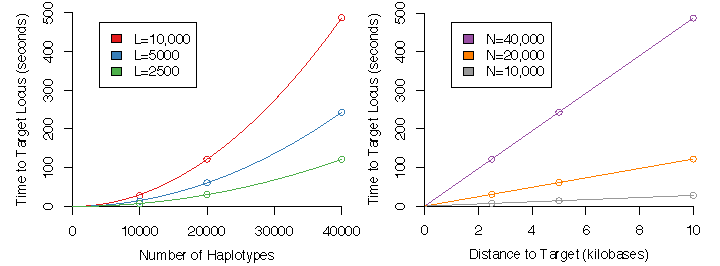
\includegraphics{fig2}
	\caption{
	  \pkg{kalis} shows the expected order $N^2$ and order $L$ scaling of the LS model.
	  Computed on an Amazon Web Services \texttt{c4.8xlarge} instance (36 vCPUs, 60 GB of RAM).
	}
	\label{fig:perfscaling}
\end{figure}

We turn now to the benefits \pkg{kalis} does provide.

Firstly, for some of the reasons highlighted in the previous Section, \pkg{kalis} exhibits accelerated performance when propagating the forward/backward recursions over more extended stretches of the genome.
This is because every effort has been made to be cache efficient, so that when more than a single variant step is taken, the strong cache locality design ensures that we are not memory bandwidth limited.
This effect can be seen quite dramatically in \Cref{fig:perfdeltaL1} by the rapid decrease in compute time per variant as longer stretches are propagated.

\begin{figure}
  \centering
  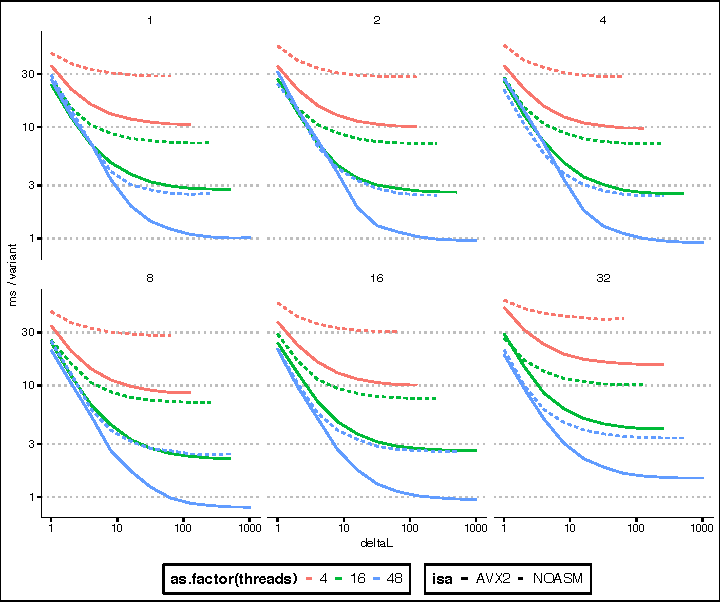
\includegraphics{fig3}
	\caption{
	  Log-log plot of milliseconds per variant performance ($y$-axis) of the forward algorithm on 10,000 haplotypes, against the number of variants propagated ($x$-axis).
	  Each panel is a different loop unrolling depth (panel title gives loop unrolling level).
	  Line colour denotes number of CPU threads, whilst a dashed line indicates vanilla \proglang{C} and a solid line indicates hand-coded AVX2 instructions.
	  In total, using AVX2, 48 threads, and loop unrolls to depth 8, it takes less than 10 seconds to propagate a $10000 \times 10000$ forward table over 10,000 variants.
	}
	\label{fig:perfdeltaL1}
\end{figure}

Secondly, the hard-coded loop unrolling functionality which can be controlled at compile time by the user can be seen to be beneficial in \Cref{fig:perfdeltaL1}.
Clearly excessive loop unrolling is harmful, with depth 32 unrolls actually being substantially slower than no unrolling.
However, unrolling to depth 8 does give a clear improvement.
The best choice of unrolls will be both problem and architecture dependent, so we recommend testing different unroll levels on the target problem before performing long compute runs.

\Cref{fig:perfdeltaL1} also illustrates that the hand-designed use of low-level vector SIMD instructions is not superfluous, with substantial speed-up afforded by their use (the difference between dashed and solid lines of the same colour).

Finally, \Cref{fig:perfdeltaL2} shows that in certain very large problem settings \pkg{kalis}' ability to pin threads can make a substantial difference.
In this setting, AVX2 showed the greatest benefit from eliminating context switching, ensuring that the cache is not invalidated by threads migrating between cores.
The lack of substantial difference between AVX2 and AVX-512 here once thread pinning is employed calls for some investigation, though this may be a result of thermal/power throttling which is known to occur especially for AVX-512 heavy code \citep{schone2019energy}.

\begin{figure}
  \centering
  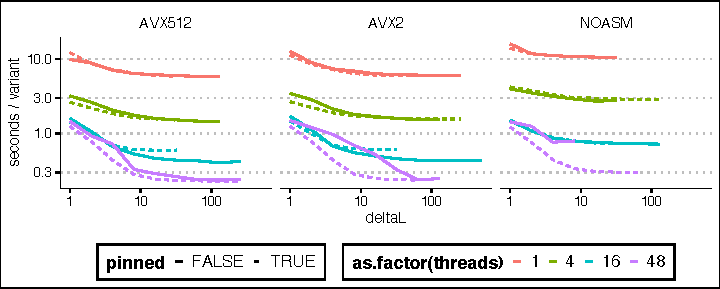
\includegraphics{fig4}
	\caption{
	  Log-log plot of seconds per variant performance ($y$-axis) of the forward algorithm on 100,000 haplotypes, against the number of variants propagated ($x$-axis).
	  Each panel is a different instruction set (AVX-512/AVX2/none).
	  Line colour denotes number of CPU threads, whilst a dashed line indicates pinned threads and a solid line indicates no thread pinning.
	  In total, using AVX-512, 48 threads, and pinned threads, it takes less approximately 38 minutes to propagate a $100000 \times 100000$ forward table over 10,000 variants.
	}
	\label{fig:perfdeltaL2}
\end{figure}

These performance examples again highlight the importance of pilot benchmark runs with different configurations of instruction set and unroll settings before embarking on long compute runs to ensure the greatest compute efficiency is achieved for a given problem and compute architecture.



\subsection*{Real-data example: recent selection for lactase persistence}
\label{sec:realdata}

\emph{LCT} is a gene on chromosome 2 that encodes lactase, the enzyme responsible for the breakdown and digestion of lactose, the sugar commonly found in milk.
Ancestral humans had a regulatory `switch' on chromosome 2 that stops lactase production after infancy when children would be weaned off breast milk.
Mutations that disrupt this switch allow lactase production to persist into adulthood, conferring a lifelong ability to extract energy from milk \cite{ingram2009lactose}.
Such mutations have arisen independently at least twice in human history, in Europe and in East Africa, and are among the strongest examples of recent positive natural selection in humans \cite{ranciaro2014genetic, bersaglieri2004genetic}.
These mutations have been shown to spread across standard human population boundaries.
Using another implementation of the LS model, \cite{busby2017inferring} estimated that a European haplotype conferring lactase persistence became prevalent within the West African Fula population due to natural selection sometime over the past two thousand years.

Here we run \pkg{kalis} on 5008 haplotypes from the 1000 Genomes Phase 3 release to revisit the haplotype structure around \emph{LCT}; the haplotypes are sampled from 26 sub-populations all over the world \cite{10002015global}.
\Cref{fig:lct} shows a clustered version of a distance matrix, calculated as in \Cref{eq:distmat}, at a variant in the regulatory region of \emph{LCT} (\texttt{rs4988235}).
To see if we could observe a pattern of gene-flow into or out of Africa similar to what was observed by \cite{busby2017inferring}, we use average pairwise linkage \cite{sokal1958statistical} to cluster the African haplotypes separately from the non-African haplotypes.
In \Cref{fig:lct}, distances between African haplotypes are shown in the upper left corner; non-African haplotypes, in the lower right corner.

\begin{figure}
  \centering
  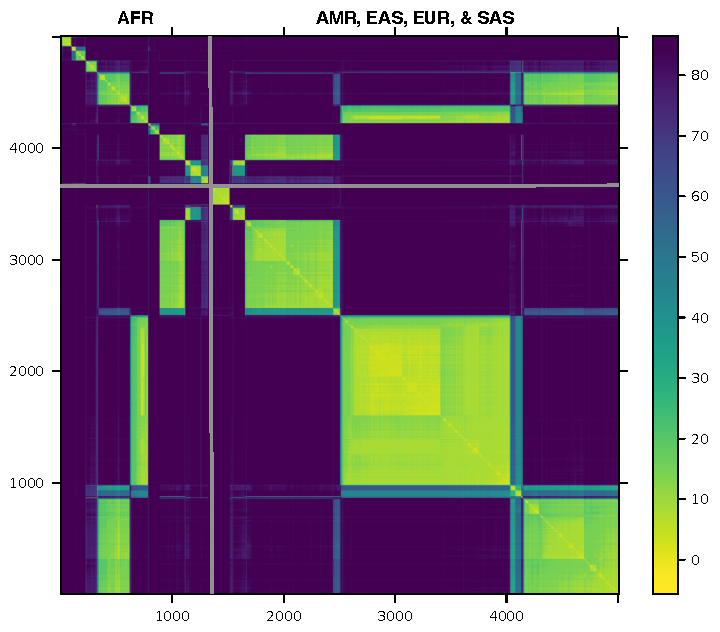
\includegraphics{fig5}
	\caption{
	  Distance matrix among 5008 haplotypes calculated at \texttt{rs4988235}, upstream of \emph{LCT}.
	  African haplotypes are clustered in the upper left corner and separated by grey lines from non-African haplotypes from the Americas (AMR), East Asia (EAS), Europe (EUR), and SAS (South Asia).
	  The scale on the right maps the colours to distances.
	}
	\label{fig:lct}
\end{figure}

Rather than 26 clusters reflecting the 26 sampled human populations, we see that there are three very distinct lactase haplotypes that are common both within and outside Africa.
This suggests that these three haplotypes, under strong positive selection pressure, recently spread across population boundaries and presumably confer lactase persistence.
However, these three haplotypes are not the only structure we see: in the upper left corner of the African (AFR) block we see some haplotypes that are only found inside Africa; and in the non-African block, a haplotype that is only found outside Africa.
We can also see some sub-structure within the clear haplotype blocks.



\section*{Discussion}
\label{sec:thepkg}

In the User Guide (Additional file 2), we introduce the package from a user perspective, from package installation right through to decoding a single variant position in \proglang{R} using \pkg{kalis}.

There are many avenues for future research in developing \pkg{kalis}.
On the model side, for example, allowing for different recombination rates between sub-populations as done in fastPHASE \cite{scheet2006fast} would be a natural extension.

On the computational side, ARM scalable vector extensions \cite{armsve} represent an interesting new approach to SIMD instruction sets, where the width of instructions need not be hard coded prior to compilation.
At present it is not widely available, but as this rolls out, it would be natural to extend \pkg{kalis} to enable targeting this new instruction set.

An important utility extension is expanding the file formats that \pkg{kalis} can natively read via \texttt{CacheHaplotypes()}, to enable simpler and more streamlined software pipelines when bioinformaticians incorporate \pkg{kalis} into their workflows.

Finally, a future avenue of potential development is extension of \pkg{kalis} to support GPU or tensor cards.
Note that it was an explicit design choice to initially target CPU SIMD extensions, since the vast majority of University high performance computing clusters have a huge amount of untapped compute power in this form, but often much more limited availability of specialist extension cards.
Therefore, by pushing performance as extensively as possible via CPU only means, we provide the greatest potential impact for end users.
This does not preclude future versions adding support for add-on compute cards.



\section*{Conclusion}

\pkg{kalis} provides a \proglang{R} interface to a highly optimized \proglang{C} implementation of the LS model that enables local ancestry, selection, and associations studies in modern large genomic datasets.



\section*{Availability and requirements}

\begin{description}
	\item[\textbf{Project name:}] \pkg{kalis}
	\item[\textbf{Project home page:}] \url{https://kalis.louisaslett.com/}
	\item[\textbf{Operating system(s):}] Linux, MacOS, Windows
	\item[\textbf{Programming language:}] \proglang{R}, \proglang{C}
	\item[\textbf{Other requirements:}] R ($\geq$ 3.5.0)
	\item[\textbf{License:}] GPL ($\geq$ 3)
	\item[\textbf{Any restrictions to use by non-academics:}] None beyond GPL ($\geq$ 3).
\end{description}



\section*{List of abbreviations}

\noindent
LS model = Li \& Stephens model

\noindent
HMM = hidden Markov model

\noindent
SIMD = single instruction, multiple data



\backmatter

\bmhead{Supplementary information}

\bmhead{Additional file 1}
\texttt{Additional\_file\_1.pdf}\\
File format: pdf \\
Title of data: Appendix \\
An appendix to the main paper containing: full mathematical derivation of the reformulation for the hidden Markov model; detailed guidance on package compilation options and installation; explanation of the HDF5 file format supported by the package.
\bmhead{Additional file 2}
\texttt{Additional\_file\_2.pdf}\\
File format: pdf \\
Title of data: User Guide \\
A tutorial-style introduction to using \pkg{kalis}, including: installation and package loading; overview of the package API; loading haplotype data; specifying Li \& Stephens model parameters; setting up hidden Markov model storage; running the Li \& Stephens model; and an example of decoding a single variant.



\section*{Declarations}

\bmhead{Ethics approval and consent to participate}

Not applicable.

\bmhead{Consent for publication}

Not applicable.

\bmhead{Availability of data and materials}

The package source code repository is at \url{https://github.com/louisaslett/kalis}.
All scripts for reproducing the results of this paper are available in this repository \url{https://github.com/louisaslett/kalis-bmc}.
The two external dependencies are: 1000 Genomes data which are available for download from \url{https://www.internationalgenome.org/}; and the msprime simulator, which may be downloaded from \url{https://tskit.dev/software/msprime.html}.

\bmhead{Competing interests}

The authors declare that they have no competing interests.

\bmhead{Funding}

This project was supported by the NHGRI Centers for Common Disease Genomics grant (UM1-HG008853), active from 2015-2022.

\bmhead{Authors' contributions}

LA architected and wrote the C-core.
LA and RC collaborated on the R interface.
RC conducted the real-world lactase persistence example.
LA and RC wrote and approved the final manuscript.

\bmhead{Acknowledgements}

Both authors would like to acknowledge Professor Ira Hall, Professor Chris Holmes, and Dr Chris Spencer for their discussions and advice on this project.



%%===========================================================================================%%
%% If you are submitting to one of the Nature Portfolio journals, using the eJP submission   %%
%% system, please include the references within the manuscript file itself. You may do this  %%
%% by copying the reference list from your .bbl file, paste it into the main manuscript .tex %%
%% file, and delete the associated \verb+\bibliography+ commands.                            %%
%%===========================================================================================%%

%\bibliography{kalis}% common bib file

\begin{thebibliography}{10}
\expandafter\ifx\csname url\endcsname\relax
  \def\url#1{\burl{#1}}\fi
\expandafter\ifx\csname urlprefix\endcsname\relax\def\urlprefix{URL }\fi
\providecommand{\bibinfo}[2]{#2}
\providecommand{\eprint}[2][]{\url{#2}}
\providecommand{\doi}[1]{\url{https://doi.org/#1}}
\bibcommenthead

\bibitem{Li2213}
\bibinfo{author}{Li, N.} \& \bibinfo{author}{Stephens, M.}
\newblock \bibinfo{title}{Modeling linkage disequilibrium and identifying recombination hotspots using single-nucleotide polymorphism data}.
\newblock \emph{\bibinfo{journal}{Genetics}} \textbf{\bibinfo{volume}{165}}, \bibinfo{pages}{2213--2233} (\bibinfo{year}{2003}).
\newblock \urlprefix\url{http://www.genetics.org/content/165/4/2213}.

\bibitem{speidel}
\bibinfo{author}{Speidel, L.}, \bibinfo{author}{Forest, M.}, \bibinfo{author}{Shi, S.} \& \bibinfo{author}{Myers, S.~R.}
\newblock \bibinfo{title}{A method for genome-wide genealogy estimation for thousands of samples}.
\newblock \emph{\bibinfo{journal}{Nature Genetics}} \textbf{\bibinfo{volume}{51}}, \bibinfo{pages}{1321--1329} (\bibinfo{year}{2019}).

\bibitem{Song1005}
\bibinfo{author}{Song, Y.~S.}
\newblock \bibinfo{title}{{Na Li and Matthew Stephens on Modeling Linkage Disequilibrium}}.
\newblock \emph{\bibinfo{journal}{Genetics}} \textbf{\bibinfo{volume}{203}}, \bibinfo{pages}{1005--1006} (\bibinfo{year}{2016}).
\newblock \urlprefix\url{http://www.genetics.org/content/203/3/1005}.

\bibitem{lawson2012inference}
\bibinfo{author}{Lawson, D.~J.}, \bibinfo{author}{Hellenthal, G.}, \bibinfo{author}{Myers, S.} \& \bibinfo{author}{Falush, D.}
\newblock \bibinfo{title}{Inference of population structure using dense haplotype data}.
\newblock \emph{\bibinfo{journal}{PLoS genetics}} \textbf{\bibinfo{volume}{8}}, \bibinfo{pages}{e1002453} (\bibinfo{year}{2012}).

\bibitem{R}
\bibinfo{author}{{R Core Team}}.
\newblock \emph{\bibinfo{title}{R: A Language and Environment for Statistical Computing}}.
\newblock \bibinfo{organization}{R Foundation for Statistical Computing}, \bibinfo{address}{Vienna, Austria} (\bibinfo{year}{2023}).
\newblock \urlprefix\url{https://www.R-project.org/}.

\bibitem{sutter2005free}
\bibinfo{author}{Sutter, H.}
\newblock \bibinfo{title}{The free lunch is over: A fundamental turn toward concurrency in software}.
\newblock \emph{\bibinfo{journal}{Dr. Dobb's Journal}} \textbf{\bibinfo{volume}{30}}, \bibinfo{pages}{202--210} (\bibinfo{year}{2005}).

\bibitem{mmx}
\bibinfo{author}{Peleg, A.} \& \bibinfo{author}{Weiser, U.}
\newblock \bibinfo{title}{{MMX technology extension to the Intel architecture}}.
\newblock \emph{\bibinfo{journal}{IEEE Micro}} \textbf{\bibinfo{volume}{16}}, \bibinfo{pages}{42--50} (\bibinfo{year}{1996}).

\bibitem{intelisa}
\bibinfo{author}{{Intel Corporation}}.
\newblock \bibinfo{title}{{Intel Architecture Instruction Set Extensions and Future Features}}.
\newblock \bibinfo{type}{Tech. Rep.} \bibinfo{number}{{319433-046}} (\bibinfo{year}{2022}).

\bibitem{armneon}
\bibinfo{author}{{ARM}}.
\newblock \bibinfo{title}{{NEON Programmer's Guide}}.
\newblock \bibinfo{type}{Tech. Rep.} \bibinfo{number}{{DEN0018A ID071613}} (\bibinfo{year}{2013}).

\bibitem{pentium}
\bibinfo{author}{Alpert, D.} \& \bibinfo{author}{Avnon, D.}
\newblock \bibinfo{title}{{Architecture of the Pentium microprocessor}}.
\newblock \emph{\bibinfo{journal}{IEEE Micro}} \textbf{\bibinfo{volume}{13}}, \bibinfo{pages}{11--21} (\bibinfo{year}{1993}).

\bibitem{C18}
\bibinfo{author}{{ISO}}.
\newblock \emph{\bibinfo{title}{{ISO\slash IEC 9899:2018 Information technology --- Programming languages --- C}}} \bibinfo{edition}{Fourth} edn (\bibinfo{publisher}{{BSI}}, \bibinfo{year}{2018}).
\newblock \urlprefix\url{https://www.iso.org/standard/74528.html}.

\bibitem{rabiner1989tutorial}
\bibinfo{author}{Rabiner, L.~R.}
\newblock \bibinfo{title}{{A tutorial on hidden Markov models and selected applications in speech recognition}}.
\newblock \emph{\bibinfo{journal}{Proceedings of the IEEE}} \textbf{\bibinfo{volume}{77}}, \bibinfo{pages}{257--286} (\bibinfo{year}{1989}).

\bibitem{schone2019energy}
\bibinfo{author}{Sch{\"o}ne, R.}, \bibinfo{author}{Ilsche, T.}, \bibinfo{author}{Bielert, M.}, \bibinfo{author}{Gocht, A.} \& \bibinfo{author}{Hackenberg, D.}
\newblock \bibinfo{editor}{{IEEE}} (ed.) \emph{\bibinfo{title}{{Energy efficiency features of the Intel Skylake-SP processor and their impact on performance}}}.
\newblock (ed.\bibinfo{editor}{{IEEE}}) \emph{\bibinfo{booktitle}{2019 International Conference on High Performance Computing \& Simulation (HPCS)}}, \bibinfo{pages}{399--406} (\bibinfo{year}{2019}).

\bibitem{ingram2009lactose}
\bibinfo{author}{Ingram, C.~J.}, \bibinfo{author}{Mulcare, C.~A.}, \bibinfo{author}{Itan, Y.}, \bibinfo{author}{Thomas, M.~G.} \& \bibinfo{author}{Swallow, D.~M.}
\newblock \bibinfo{title}{Lactose digestion and the evolutionary genetics of lactase persistence}.
\newblock \emph{\bibinfo{journal}{Human genetics}} \textbf{\bibinfo{volume}{124}}, \bibinfo{pages}{579--591} (\bibinfo{year}{2009}).

\bibitem{ranciaro2014genetic}
\bibinfo{author}{Ranciaro, A.} \emph{et~al.}
\newblock \bibinfo{title}{{Genetic origins of lactase persistence and the spread of pastoralism in Africa}}.
\newblock \emph{\bibinfo{journal}{The American Journal of Human Genetics}} \textbf{\bibinfo{volume}{94}}, \bibinfo{pages}{496--510} (\bibinfo{year}{2014}).

\bibitem{bersaglieri2004genetic}
\bibinfo{author}{Bersaglieri, T.} \emph{et~al.}
\newblock \bibinfo{title}{Genetic signatures of strong recent positive selection at the lactase gene}.
\newblock \emph{\bibinfo{journal}{The American Journal of Human Genetics}} \textbf{\bibinfo{volume}{74}}, \bibinfo{pages}{1111--1120} (\bibinfo{year}{2004}).

\bibitem{busby2017inferring}
\bibinfo{author}{Busby, G.} \emph{et~al.}
\newblock \bibinfo{title}{{Inferring adaptive gene-flow in recent African history}}.
\newblock \emph{\bibinfo{journal}{BioRxiv}} \bibinfo{pages}{205252} (\bibinfo{year}{2017}).

\bibitem{10002015global}
\bibinfo{author}{Consortium, . G.~P.} \emph{et~al.}
\newblock \bibinfo{title}{A global reference for human genetic variation}.
\newblock \emph{\bibinfo{journal}{Nature}} \textbf{\bibinfo{volume}{526}}, \bibinfo{pages}{68} (\bibinfo{year}{2015}).

\bibitem{sokal1958statistical}
\bibinfo{author}{Sokal, R.~R.}
\newblock \bibinfo{title}{A statistical method for evaluating systematic relationships.}
\newblock \emph{\bibinfo{journal}{Univ. Kansas, Sci. Bull.}} \textbf{\bibinfo{volume}{38}}, \bibinfo{pages}{1409--1438} (\bibinfo{year}{1958}).

\bibitem{scheet2006fast}
\bibinfo{author}{Scheet, P.} \& \bibinfo{author}{Stephens, M.}
\newblock \bibinfo{title}{A fast and flexible statistical model for large-scale population genotype data: applications to inferring missing genotypes and haplotypic phase}.
\newblock \emph{\bibinfo{journal}{The American Journal of Human Genetics}} \textbf{\bibinfo{volume}{78}}, \bibinfo{pages}{629--644} (\bibinfo{year}{2006}).

\bibitem{armsve}
\bibinfo{author}{Stephens, N.} \emph{et~al.}
\newblock \bibinfo{title}{{The ARM Scalable Vector Extension}}.
\newblock \emph{\bibinfo{journal}{IEEE Micro}} \textbf{\bibinfo{volume}{37}}, \bibinfo{pages}{26--39} (\bibinfo{year}{2017}).

\end{thebibliography}



\end{document}
